\graphicspath{  {mainmatter/Freed_2012/} }

\title*{2012: The Fingerphone: a Case Study of Sustainable Instrument Redesign}
\titlerunning{Sustainable Instrument Redesign}
\author{Adrian Freed}
\authorrunning{Freed}

%\institute{Adrian Freed\at CNMAT, UC Berkeley, 1750 Arch Street, Berkeley, CA 94709, \email{adrian@cnmat.berkeley.edu}}
%
%
\maketitle

\abstract*{The Fingerphone, a reworking of the Stylophone in conductive paper, is presented as an example of new design approaches for sustainability and playability of electronic musical instruments.}

\section{Introduction}


\begin{figure}[t]
\centering
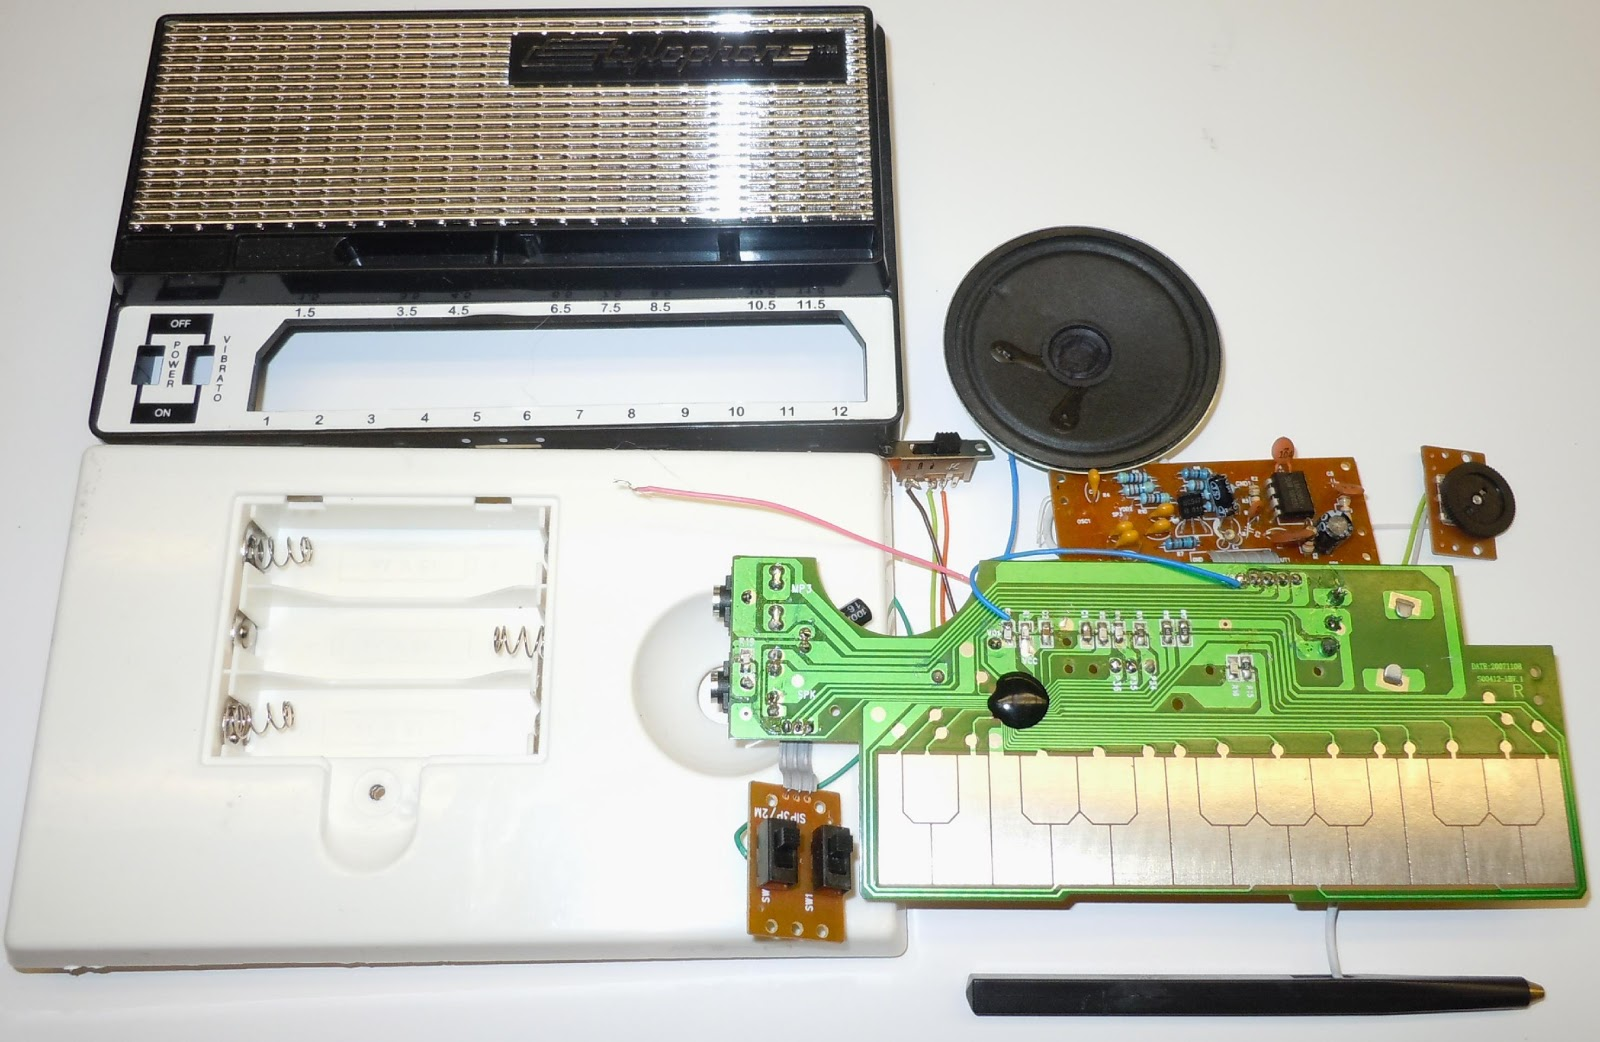
\includegraphics[width=\textwidth]{fig1.jpg}
\caption{The Disassembled Stylophone.}
\label{Freed:img-1}
\end{figure}



\subsection{Stylophone}

The Stylophone is a portable electronic musical instrument that was commercialized in the 1970's and enjoyed a brief success primarily in the UK. This is largely attributable to its introduction on TV by Rolf Harris, its use in the song that launched David Bowie's career, ``Space Oddity,'' and its appearance in a popular TV series ``The Avengers.'' Three million instruments were sold by 1975. A generation later the product was relaunched. The artist ``Little Boots'' has prompted renewed interest in the product by showcasing it in her hit recording ``Meddle.''

\subsection{Mottainai! (What a waste!)}

The Stylophone in its current incarnation is wasteful in both its production and interaction design. The new edition has a surprisingly high parts count, material use and carbon footprint. The limited affordances of the instrument waste the efforts of most who try to learn to use it.

Musical toy designers evaluate their products according to MTTC (Mean Time to Closet), and by how many battery changes consumers perform before putting the instrument aside \cite{Capps:2011}. Some of these closeted instruments reemerge a generation later when ``old'' becomes the new ``new''---but most are thrown away.

This paper addresses both aspects of this waste by exploring a rethinking and redesign of the Stylophone, embodied in a new instrument called the Fingerphone.

\subsection{History}

The Stylophone was not the first stylus-based musical instrument. Professor Robert Watson of the University of Texas built an ``electric pencil'' in 1948 \cite{Anonymous:1948}. The key elements for a wireless stylus instrument are also present in the David Grimes patent of 1931 \cite{Anonymous:1948} including conductive paper and signal synthesis from position-sensing potentiometers in the pivots of the arms of a pantograph. Wireless surface sensing like this wasn't employed commercially until the GTCO Calcomp Interwrite's Schoolpad of 1981.

Electronic musical instruments like the Fingerphone with unencumbered surface interaction were built as long ago as 1748 with the Denis d'Or of V\'{a}clav Prokop Divi\v{s}. Interest in and development of such instruments continued with those of Elisha Gray in the late 1800's, Theremin in the early 1900's, Eremeeff, Trautwein, Lertes, Heller in the 1930's, Le Caine in the 1950's, Michel Waisvisz and Don Buchla in the 1960's, Salvatori Martirano and the circuit benders in the 1970's \cite{Roads:1996a}.

\subsection{Contributions}

The basic sensing principle, sound synthesis method and playing style of the
Stylophone and Fingerphone are well known so the novel aspects of the work
presented here are in the domain of the tools, materials, form and design methods
with which these instruments are realized.

Contributions of the paper include: a complete musical instrument
design that exploits the potential of paper sensors, a novel strip origami
pressure sensor, surface e-field sensing without external passive components, a
new manual layout to explore sliding finger gestures, and suggestions of how to
integrate questions of sustainability and longevity into musical instrument
design and construction.

\section{The Fingerphone}

\subsection{Reduce}

The Fingerphone (Figure~\ref{Freed:img-2}) achieves low total material use, low energy cost and
a small carbon footprint by using comparatively thin materials, recycled
cellulose and carbon to implement the functions of the Stylophone without its
high-energy cost and toxic materials: plastics, metals, glass fiber and resins.

\begin{figure}[t]
\centering
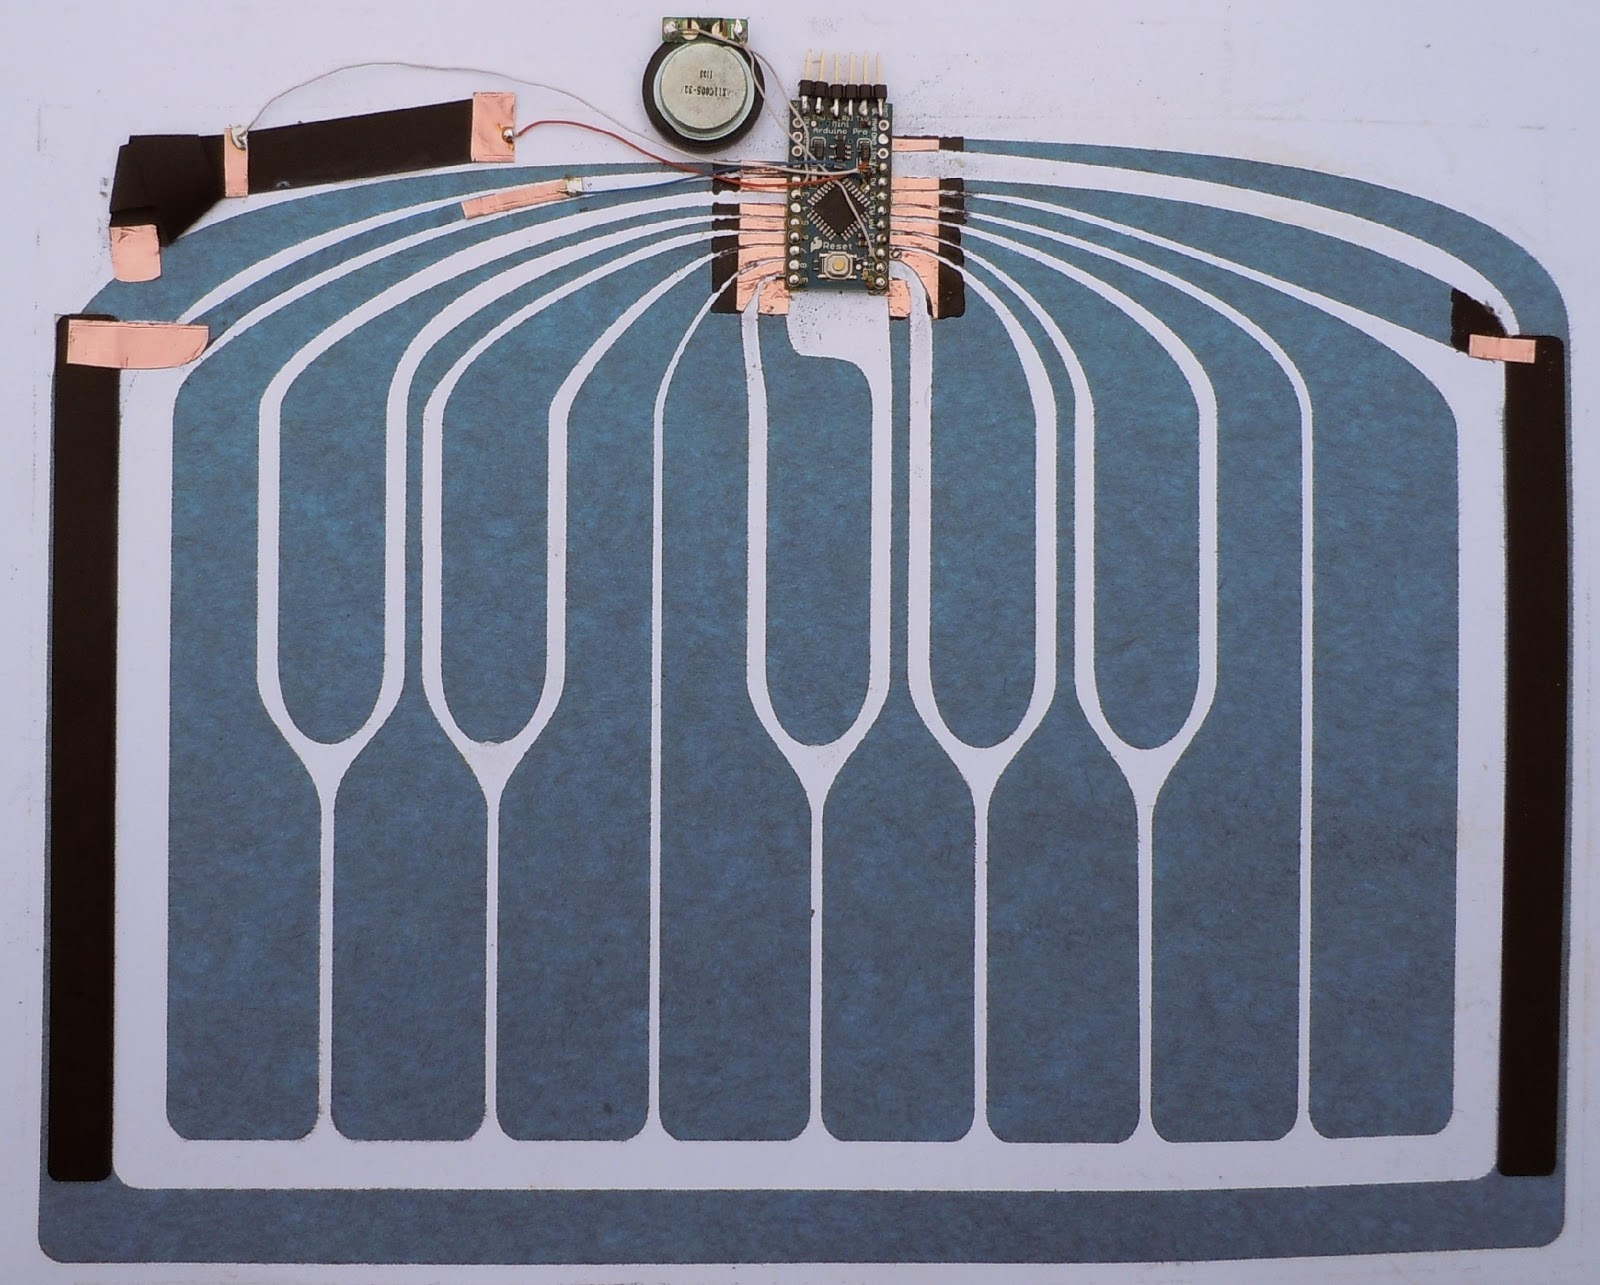
\includegraphics[width=\textwidth]{fig2}
\caption{The Fingerphone.}
\label{Freed:img-2}
\end{figure}


The Stylophone contains two major, separate circuit boards with a
different integrated circuit on each: one for the oscillator and stylus-board,
the other for an LM386 power amplifier for the small speaker. The Fingerphone has
only one integrated circuit, an Atmel 8-bit micro-controller, that is used to
sense e-field touch and pressure on paper transducers, synthesize several digital
oscillators and drive the sound transducer using an integrated pulse width
modulation controller (PWM) as an energy-efficient, inductor-less class D
amplifier.

The Fingerphone's playing surface, switches and volume control
functions are achieved using conductive paper \cite{Koehly:2006,Koehly:2011}. Various other materials
were explored including embroidered silver plaited nylon thread (Figure~\ref{Freed:img-3}a), and a
water-based silk-screened carbon-loaded ink (Figure~\ref{Freed:img-3}b).
Paper is an interesting choice because cellulose, its core
component, is the most common polymer, one that can be harvested sustainably and
is also readily available as a recycled product.

\begin{figure}[t]
\centering
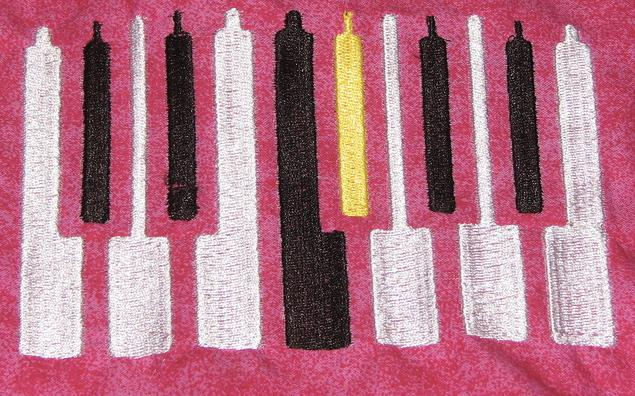
\includegraphics[height=35mm]{fig3}
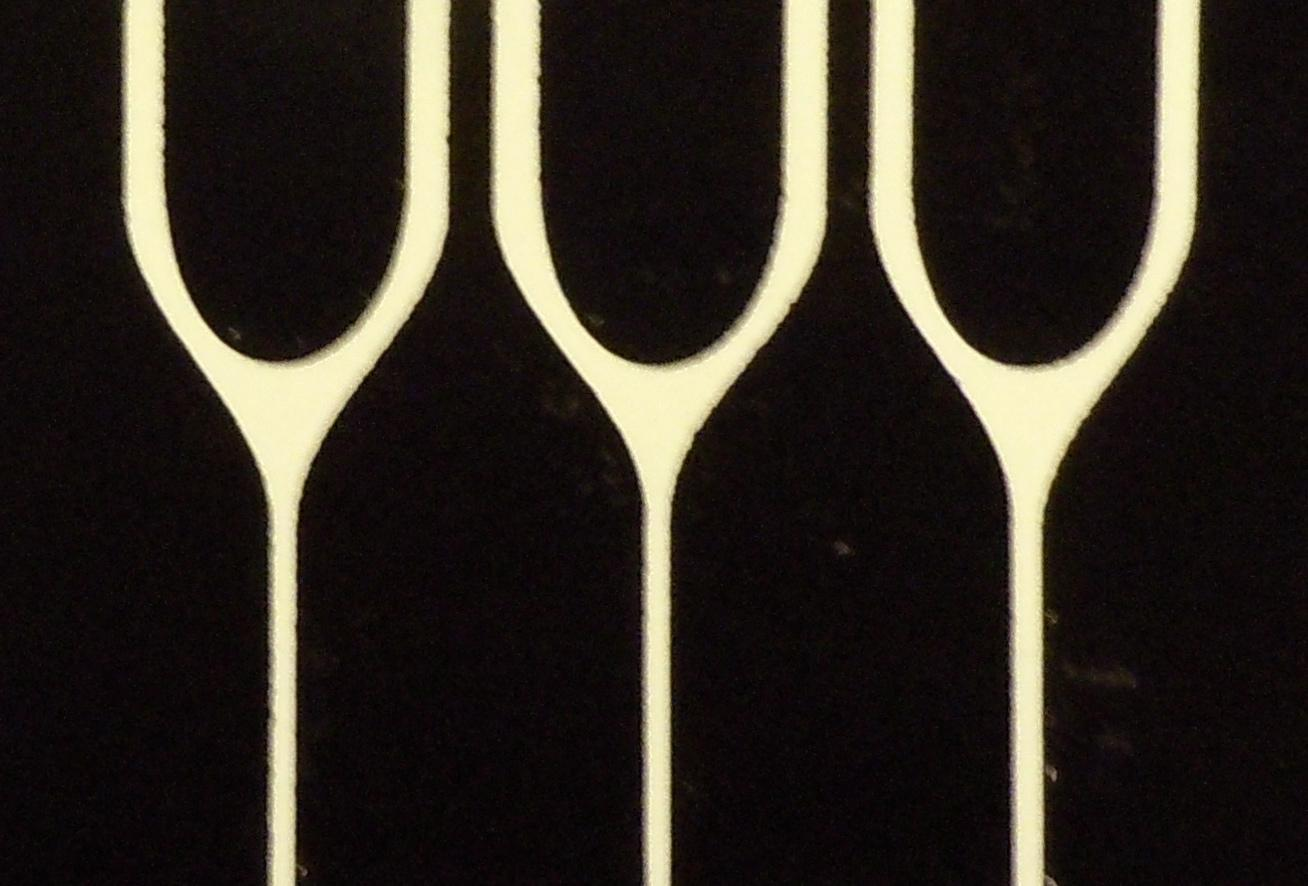
\includegraphics[height=35mm]{fig4}
\caption{(a) Embroidered manual, (b) printed manual.}
\label{Freed:img-3}
\end{figure}

Complete carbon footprint, and lifecycle cost analyses are
notoriously hard to do well but we can use some simple measures as proxies: The
Stylophone has 65 components, a production Fingerphone would have only six.
Manufacturing process temperature is another useful proxy: the Stylophone's
metals, plastic and solder suggest a much higher cost than those associated with
paper. At first glance it would appear that the waste stream from the paper of
the Fingerphone might be more expensive than the Stylophone. In fact they are
similar because of the packaging of the reels the surface mount parts are
contained in during manufacturing of the Stylophone. The Fingerphone waste paper
stream can be recycled back into future Fingerphones.

In some products, such as grocery bags, plastic compares favorably
to paper in terms of environmental impact and production energy budgets.  Paper
has the advantage in musical instrument s such as the Fingerphone of providing a
medium to inscribe multiple functions---a plurifunctionality difficult to achieve
with plastics or metals. These functions include: visual and tactile fiducials
for the performer, highly conductive and insulating regions for the playing
surface, a membrane for the bending wave sound transducer and an absorbent and
thermally insulating substrate for connections and support of the
micro-controller and output transducer. This plurifunctionality is found in
traditional fretted chordophones: frets serve as fiducials, to define the length
of the sounding string, as a fulcrum for tension modulation of the string and as
an anvil to transfer energy to the string in the ``hammer on'' gesture.

Capacitive sensing of the performer's digits obviates the need for
the Stylophone's metal wand and connecting wire entirely. Employing a
distributed-mode driver eliminates the need for a loudspeaker cone and metal
frame. In this way the entire instrument surface can be used as an efficient
radiator.

The prototype of Figure~\ref{Freed:img-2} uses a small, readily available printed
circuit board for the Atmel micro-controller; the production version would
instead use the common ``chip on board'' technique observable as a black patch of
epoxy on the Stylophone oscillator board, on cheap calculators and other high
volume consumer products. This technique has been successfully used already for
paper and fiber substrates as in Figure~\ref{Freed:img-5}a \cite{Yoo:2009}.


% ARJ: Poor image quality, so I have merged this into one figure.
\begin{figure}[t]
\centering
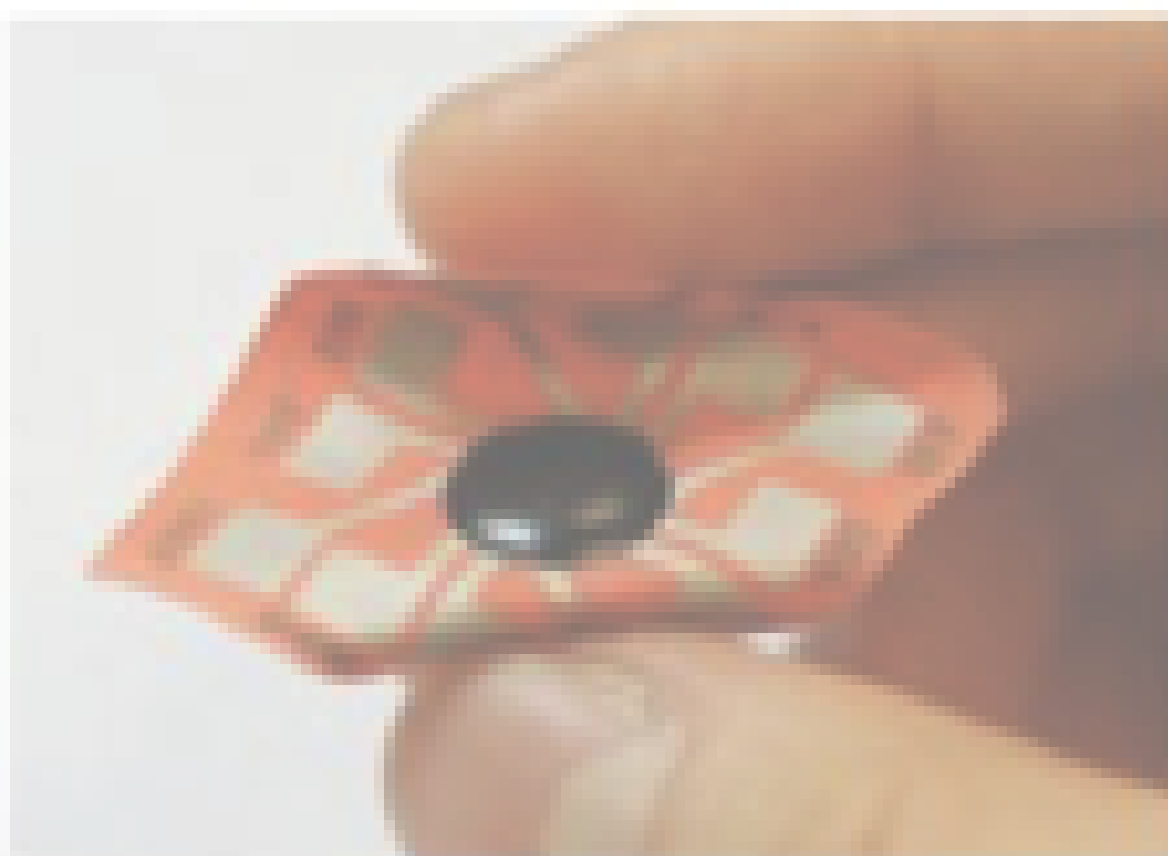
\includegraphics[height=25mm]{fig5}
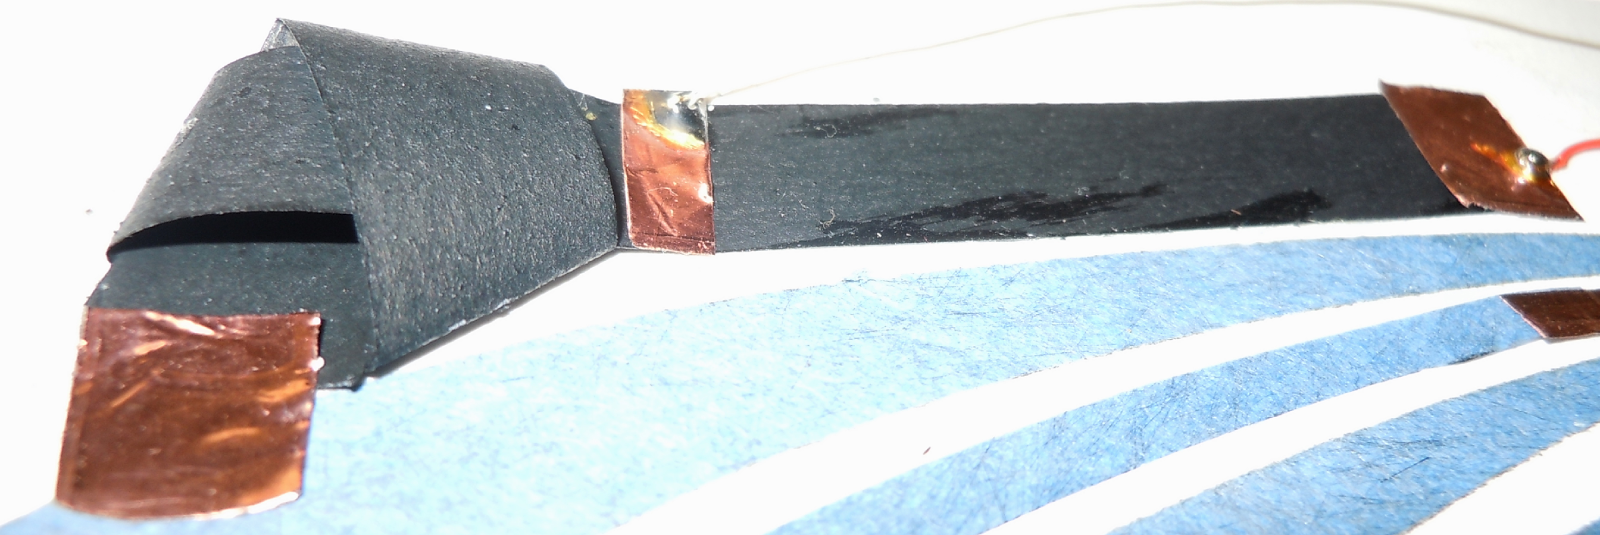
\includegraphics[height=25mm]{fig6}
\caption{(a) Chip on Fabric, (b) Origami Force Sensor.}
\label{Freed:img-5}
\end{figure}

In conventional electronic design the cost of simple parts such as
resistors and capacitors is considered to be negligible; laptop computers, for
example, employ hundreds of these discrete surface mounted parts. This
traditional engineering focus on acquisition cost from high volume manufacturers
doesn't include the lifecycle costs and, in particular, ignores the impact of
using such parts on the ability for users to eventually recycle or dispose of the
devices. Rather than use a conventional cost rationale the Fingerphone design was
driven by the question: how can each of these discrete components be eliminated
entirely? For example, Atmel provides a software library and guide for
capacitance sensing. Their design uses a discrete resistor and capacitor for each
sensor channel. The Fingerphone uses no external resistors or capacitors. The
built-in pull-up resistors of each I/O pin are used instead in conjunction with
the ambient capacitance measured between each key and its surrounding keys.

The Stylophone has a switch to engage a fixed frequency and fixed
depth vibrato, and rotary potentiometers to adjust pitch and volume. These
functions are controlled on the Fingerphone using an origami piezoresistive
sensor and linear paper potentiometers. The former is a folded strip of paper
using a flattened thumb knot that forms a pentagon (Figure~\ref{Freed:img-5}b). Notice that 3
connections are made to this structure eliminating the need for a pull up
resistor and establishing a ratiometric measure of applied pressure.


% \begin{figure}[t]
% \centering
% 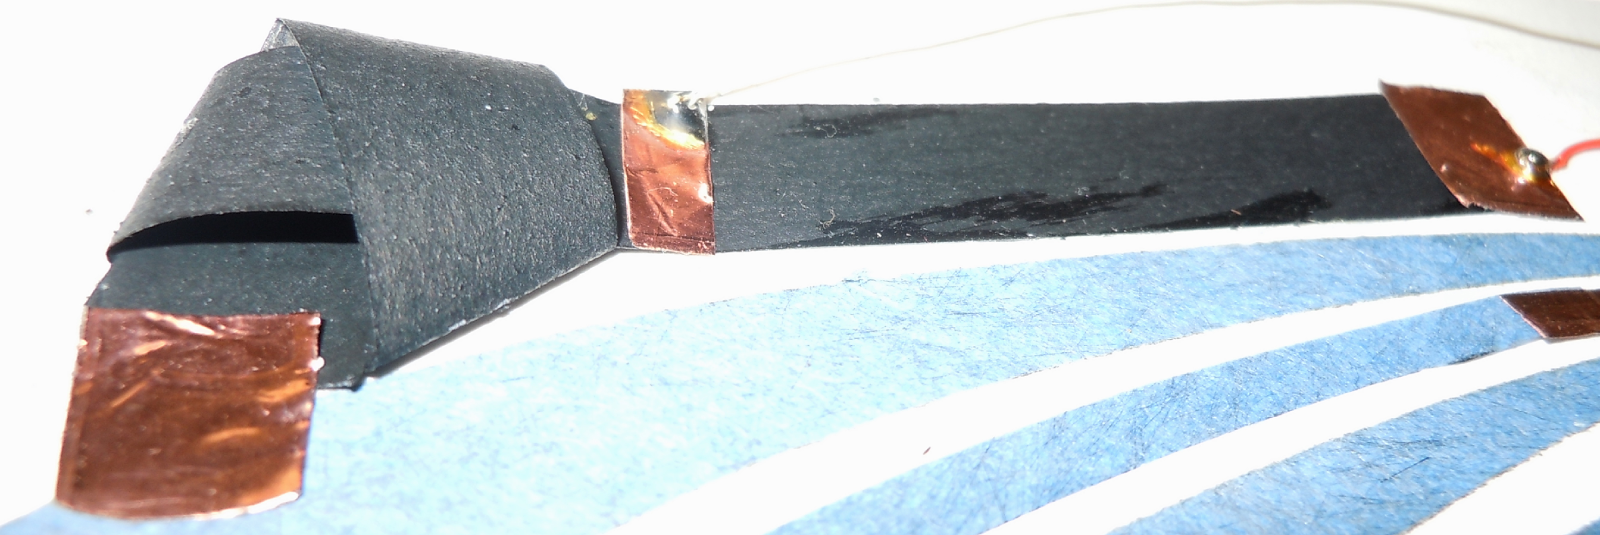
\includegraphics[width=184pt]{fig6}
% \caption{Origami Force Sensor.}
% \label{Freed:img-6}
% \end{figure}


The remaining discrete components on the micro-controller board can be
eliminated in a production version: The LED and its series resistor are used for
debugging---a function easily replaced using sound \cite{Turing:1951}. The micro-controller can
be configured to not require either a pull-up resistor or reset button and to use
an internal RC clock instead of an external crystal or ceramic resonator. This RC
clock is not as accurate as the usual alternatives but certainly is as stable as
the Stylophone oscillator. This leaves just the micro-controller's decoupling
capacitor.

The magnet of the sound transducer shown in Figure~\ref{Freed:img-2} is one of the
highest energy-cost devices in the design. A production version would use a
piezo/ceramic transducer instead. These have the advantage of being relatively
thin (1--4mm) and are now commonly used in cellphones and similar portable devices
because they don't create magnetic fields that might interfere with the compasses
now used in portable electronics. By controlling the shape of the conductive
paper connections to a piezo/ceramic transducer a low-pass filter can be tuned to
attenuate high frequency aliasing noise from the class D amplifier.

\subsection{Reuse}

Instead of the dedicated battery compartment of the Stylophone, the Fingerphone
has a USB mini connector so that an external, reusable source of power can be
connected---one that is likely to be shared among several devices, e.g,
cameras, cellphones, or laptop computers. Rechargable, emergency chargers for
cellphones that use rechargeable lithium batteries and a charging circuit are a
good alternative to a disposable battery (Figure~\ref{Freed:img-7}).


\begin{figure}[t]
\centering
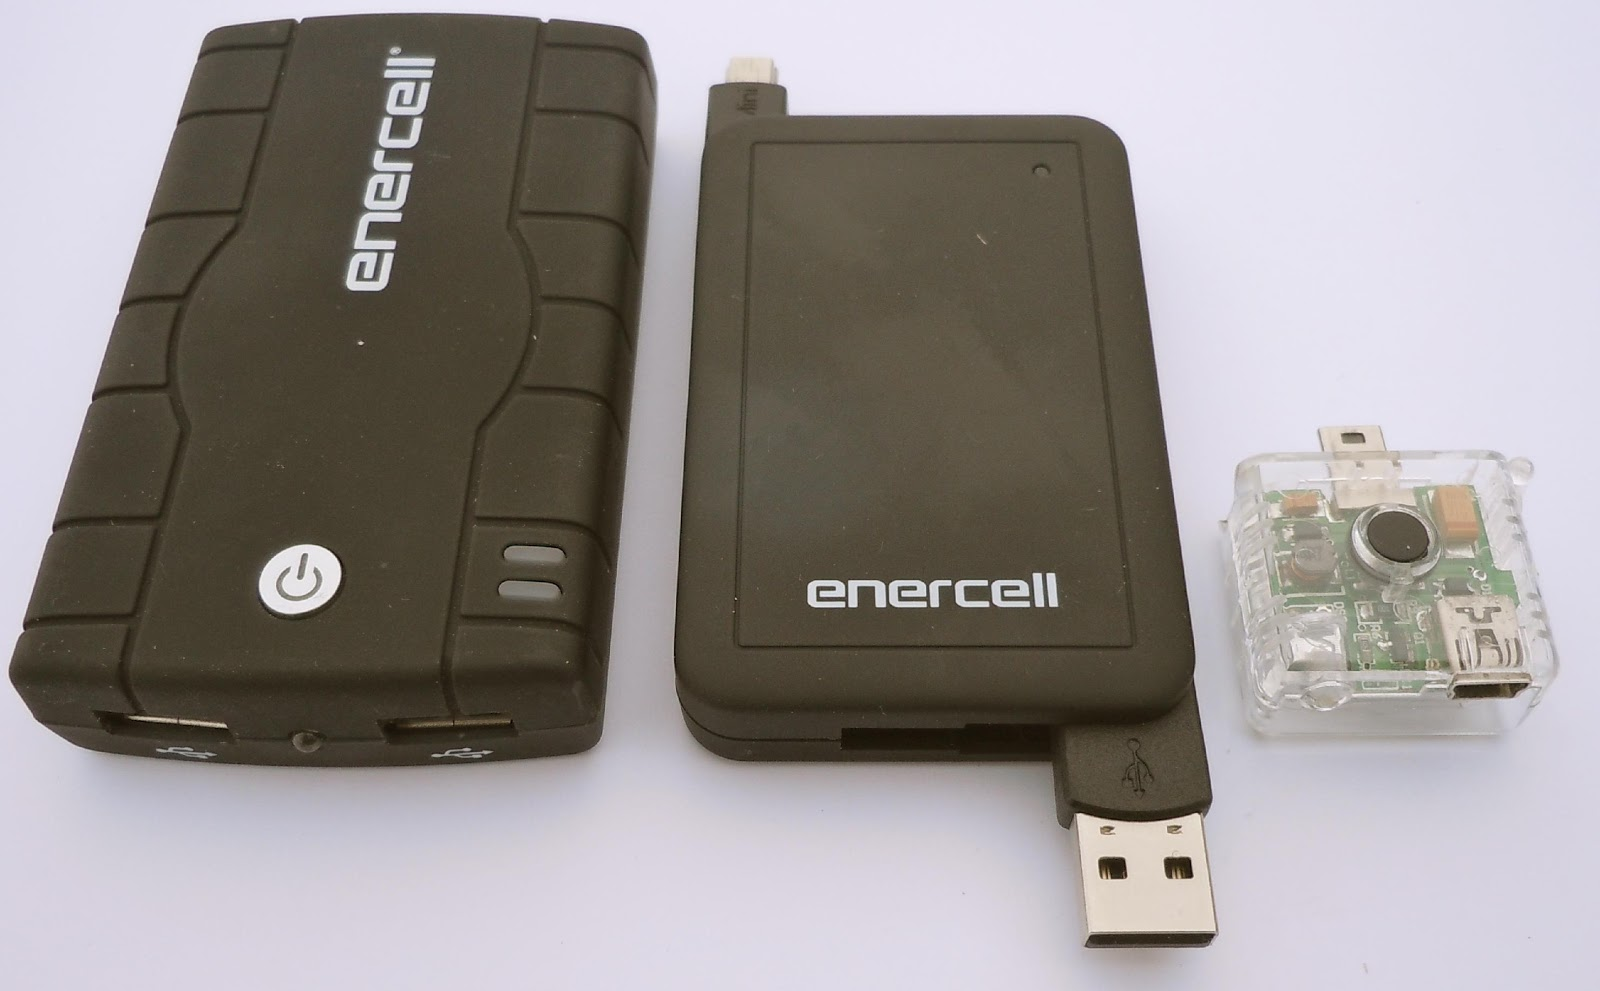
\includegraphics[width=70mm]{fig7}
\caption{Reusable Power Sources.}
\label{Freed:img-7}
\end{figure}



This approach of providing modular power sources shared between
multiple devices may be found in modern power tool rechargeable battery packs,
and in the Home Motor of 1916. This was available from the Sears mail order
catalog with attachments for sewing, buffing, grinding, and sexual stimulation
 \cite{Maines:1989}.

The Fingerphone components are installed on a light, stiff
substrate to provide a resonating surface for the bending mode transducers. This
has been found to be a good opportunity for reuse so prototype Fingerphones have
been built on the lid of a pizza box, a cigar box, and a sonic greeting card from
Hallmark---all of which would normally be discarded after their first use. Such
reuse has precedent in musical-instrument building, e.g., the cajon (cod-fish
shipping crates), the steel-pan (oil drums), and ukulele (cigar boxes).

\subsection{Recycle}

The bulk of the Fingerphone is recyclable, compostable paper. A ring of
perforations in the paper around the micro-controller would facilitate separation
of the small non-recyclable component from the recyclable paper.

\section{Use Maximization}

\subsection{Introduction}

The Stylophone has a single, strident, sawtooth-wave timbre. There is no control
over the amplitude envelope of the sawtooth wave other than to turn it off. This
guarantees (as with the kazoo, harmonica, and vuvuzela) that the instrument will
be noticed---an important aspect of the gift exchange ritual usually associated
with the instrument. This combination of a constrained timbre and dynamic
envelope presents interesting orchestration challenges.  These have been
addressed by David Bowie and Little Boots in different ways: In early recordings
of ``Space Oddity'' the Stylophone is mostly masked by rich orchestrations---in
much the way the string section of an orchestra balances the more strident
woodwinds such as the oboe. Little Boots' ``Meddle'' begins by announcing the
song's core ostinato figure, the hocketing of four staccato ``call'' notes on the
Stylophone with ``responding'' licks played on the piano. The lengths of call and
response are carefully balanced so that the relatively mellow instrument, the
piano, is given more time than the Stylophone.

\subsection{Timbre}

The oscillators of the Fingerphone compute a digital phasor using 24-bit
arithmetic and index tables that include sine and triangle waves. The phasor can
also be output directly or appropriately clipped to yield approximations to
sawtooth and square/pulse waves respectively. Sufficient memory is available for
custom waveshapes or granular synthesis. The result is greater pitch precision
and more timbral options than the Stylophone.

\subsection{Dynamics }

An envelope function, shaped according to the touch expressivity afforded by
electric field sensing, modulates the oscillator outputs of the Fingerphone. The
level of dynamic control achieved is comparable to the nine ``waterfall'' key
contacts of the Hammond B3 organ.

Legato playing is an important musical function and it requires
control of note dynamics. The audible on/off clicks of the Stylophone disrupt
legato to such an extent that the primary technique for melodic playing of the
instrument is to rapidly slide the stylus over the keys to create a perceived
blurring between melody notes. The dedicated performer with a steady hand can
exploit a narrow horizontal path half way down the Stylophone stylus-board to
achieve a chromatic run rather than the easier diatonic run

Legato in the Fingerphone is facilitated by duophony so that notes
can actually overlap---as in traditional keyboard performance. Full, multi-voice
polyphony is also possible with a faster micro-controller or by taking advantage
of remote synthesis resources driven by the OSC and MIDI streams flowing from the
Fingerphone's USB port.

\subsection{Manual Layouts}


\begin{figure}[t]
\centering
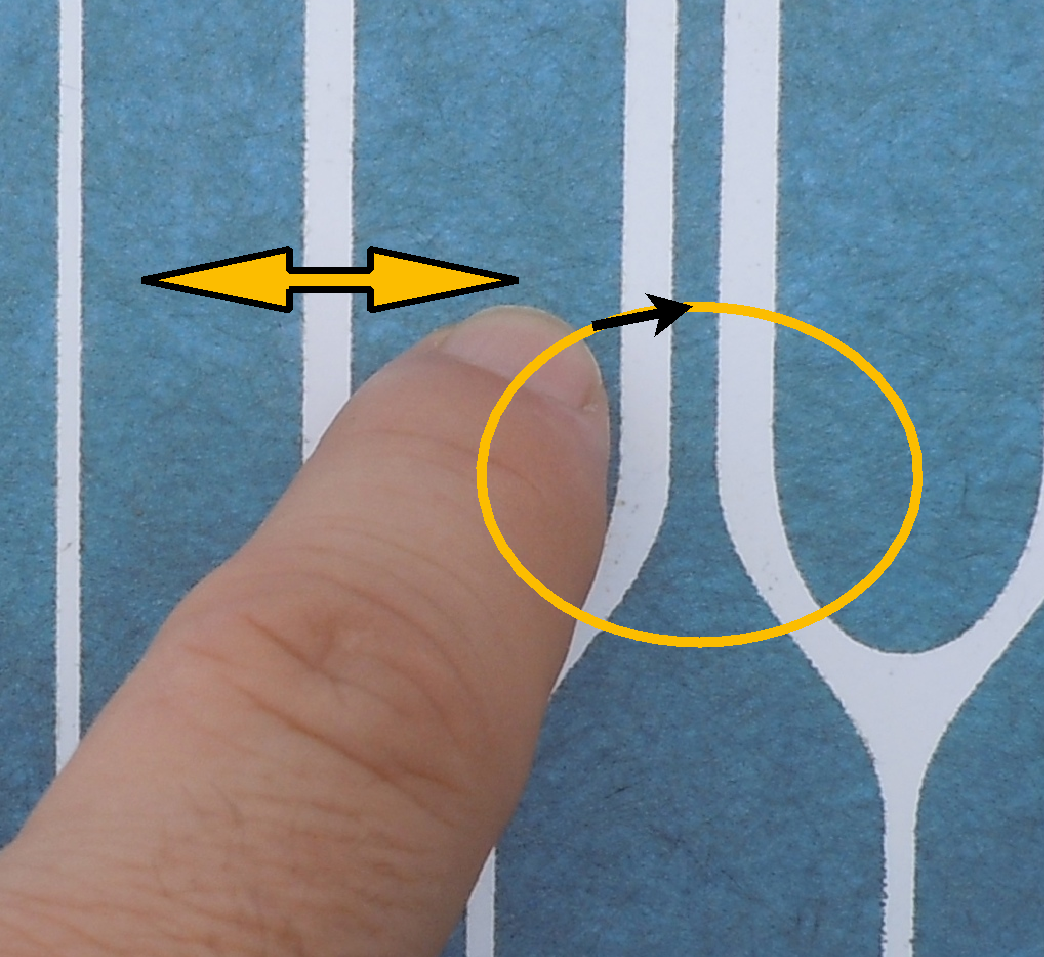
\includegraphics[width=184pt]{fig8}
\caption{Trills.}
\label{Freed:img-8}
\end{figure}



Surface interaction interfaces provide fundamentally different affordances to
those of sprung or weighted action keyboards. In particular it is slower and
harder to control release gestures on surfaces because they don't provide the
stored energy of a key to accelerate and preload the release gesture. This factor
and the ease of experimentation with paper suggest a fruitful design space to
explore: new surface layout designs. The layout illustrated in Figure~\ref{Freed:img-8} resulted
from experiments with elliptical surface sliding gestures that were inspired by
the way Dobro and lapstyle guitar players perform vibrato and trills. Various
diatonic and chromatic ascending, descending and cyclical runs and trills can be
performed by orienting, positioning and scaling these elliptical and back and
forth sliding gestures on the surface.

\subsection{Size Matters}

By scaling the layout to comfortable finger size it is possible to play the
white ``keys'' between the black ones--something that is impossible with the
Stylophone layout.

The interesting thing about modulations of size in interactive
systems is that continuous changes are experienced as qualitatively discrete,
i.e., For each performer, certain layouts become too small to reliably play or
too large to efficiently play. The economics of mass manufacturing interacts with
this in a way that historically has narrowed the number of sizes of instruments
that are made available. For example, the Jaranas of the Jarochos of Mexico are a
chordophone that players build for themselves and their children. They are made
``to measure'' with extended families typically using seven or eight different
sizes. The vast majority of manufactured guitars on the other hand are almost
entirely ``full size'' with a few smaller sizes available for certain styles.
This contrasting situation was also present with the hand-built fretless banjos
of the 19$^{th}$ century now displaced by a few sizes of manufactured, fretted
banjos.

In the case of the Stylophone the NRE (Non-recurring Engineering)
costs for two molds and the circuit boards discourage the development of a range
of sizes. There are also costs associated with the distribution and shelving in
stores of different sizes.  The lower cost structures of the Fingerphone on the
other hand allow for a wider range of sizes. Prototypes have been developed by
hand and with a cheap desktop plotter/cutter. Different scales can be
experimented with in minutes instead of the hours required to develop circuit
boards. Also, die cutting of paper is cheaper than injection molding or etching
in production.

The use of a finger-size scale would appear to put the Fingerphone
at a portability disadvantage with respect to the Stylophone.  It turns out that
fabric and paper allow for folded Fingerphones that are no larger than the
Stylophone for transport. Roll-up computer keyboards and digitizing tablets are
precedents for this approach.

\section{Discussion}

\subsection{Impact}

By itself the Fingerphone will not have a significant direct impact on the
sustainability issues the world faces. However, now that musical instrument
building is being integrated as standard exercises in design school classes, the
Fingerphone can serve as a strong signal that more environmentally responsible
materials and design techniques are available.

\subsection{Design Theory}

Simondon's thesis on the technical object \cite{Simondon:1958} describes the value  of
plurifunctionality to avoid  the pitfalls of ``hypertelic and maladapted
designs.'' Judging by the number of huge catalogs of millions of highly
functionally-specific electronic parts now available, the implications of
Simondon's philosophical study were largely ignored. The Fingerphone illustrates
how plurifunctionality provides designers with an alternative route to economies
of scale than the usual high-volume-manufacturing one where the cost of
development is amortized over a large number of inscribed functions instead of a
large number of high volume parts.

\subsection{Transitional Instruments}

The Fingerphone adds to a debate in the NIME community about accessibility, ease
of use and virtuosity. Wessel and Wright declare that it is possible to build
instruments with a low entry point and no ceiling on virtuosity \cite{Wessel:2002}. Blaine and
Fels argue that this consideration is irrelevant to casual users of collaborative
instruments \cite{Blaine:2003}. Isn't there a neglected space in between of transitional
instruments that serve people on a journey as they acquire musical skills and
experience?  Acoustic instrument examples include the melodica, ukulele and
recorder. The Stylophone, in common with Guitar hero and Paper Jamz, is designed
with a primary focus on social signaling of musical performance. The Fingerphone
shows that affordable instruments may be designed that both call attention to the
performer and also afford the exercise and development of musical skills, and a
facilitated transition to other instruments.

\begin{acknowledgement}
Thanks for support from Pixar/Disney, Meyer Sound Labs, Nathalie Dumont from the
Concordia University School of Fine Arts and the Canada Grand project.
\end{acknowledgement}


\section*{Author Commentary: My Creative Response To Three Umbridges}

\paragraph{Adrian Freed}

The Fingerphone is my creative response to three umbridges: the waste and unsustainability of musical instrument manufacturing practices, the prevailing absence of long historical research to underwrite claims of newness in NIME community projects, and the timbral poverty of the singular, strident sawtooth wavefrom of the Stylophone---the point of departure for the Fingerphone instrument design.
 
This paper is the first at NIME of my ongoing provocations to the community to enlarge what we may mean by ``new'' and ``musical expression.''  I propose a change of  scale away from  solipsistic narratives of instrument builders and players to cummunitarian accounts that celebrate plural agencies and mediations. %[Born]. 
The opening gesture in this direction is a brief historicization of the Fingerphone instrument. Avoiding the conventional trope of just differentiating this instrument from its immediate predecessors to establish ``newness,'' the Fingerphone is enjoined to two rich instrumental traditions, the histories of which are still largely unwritten: stylus instruments, and electrosomatophones.  The potential size of this iceberg is signaled by citing a rarely-cited musical stylus project from 1946 instead of the usually cited projects of the 1970's, e.g. Xenakis's UPIC or the Fairlight CMI lightpen.
 
Electrosomatophones are electronic sounding instruments that integrate people's bodies into their circuits. They are clearly attested in depictions from the eighteenth century of Stephen Gray's ``flying boy'' experiments and demonstrations, where a bell is rung by electrostatic forces produced by electric charges stored in the body of a boy suspended in silks.  Electrosomatophones appear regularly in the historical record from this period to the present day.
 
The production of Lee De Forest's audion tube is an important disruptive moment because the vacuum tube provided amplification and electrical isolation permitting loud sounds to be emitted from electrosomatophones without the pain of correspondingly large currents running through the performer's body. While the theremin is the electrosomatophone that has gained the most social traction, massification of electrosomatophone use began with the integration of capacitive multitouch sensing into cellphones, an innovation prefigured by Bill Buxton \cite{Lee:1985} and Bob Boie's \cite{Boie:1989} inventions of the mid-1980's.
 
Achieving the sustainable design properties of the Fingerphone required working against the grain of much NIME practice, especially the idea of separating controller, synthesizer and loudspeaker into their own enclosures. Such a separation might have been economical at a time when enclosures, connectors and cables were cheaper than the electronic components they house and connect but now the opposite is true. Instead of assembling a large number of cheap, specialized monofunctional components, the Fingerphone uses a plurifuctional design approach where materials are chosen, shaped and interfaced to serve many functions concurrently. The paper components of the Fingerphone serve as interacting surface, medium for inscription of fiducials, sounding board and substrate for the electronics.

The first prototype Fingerphone was built into a recycled pizza box. The version presented at the NIME conference was integrated into the poster used for the presentation itself. This continues a practice I initially have been using e-textiles for, the practice of choosing materials that give design freedoms of scale and shape instead of using rigid circuit boards and off-the-shelf sensors. This approach will continue to flourish and become more commonplace as printing techniques for organic semiconductors, sensors and batteries are massified.
 
The Fingerphone has influenced work on printed loudspeakers \cite{Rowland:2013} and the sonification of compost \cite{Parker}. Printed keyboards and speakers are now a standard application promoted by manufacturers of conductive and resistive inks.
 
In addition to providing builders with an interesting instrument design, I hope the Fingerphone work will lead more instrument builders and players to explore the nascent field of critical organology \cite{TreschDolan:2013}, deepen discourse of axiological concerns in musical instrument design, and adduce early sustainability practices that ecomusicologists will be able to study.



\section*{Expert Commentary: Pushing The Sensor Boundaries In Digital Musical Instruments}


\paragraph{Alexander Refsum Jensenius}


Of the more than 1200 papers published at the NIME conferences, Adrian Freed's paper resonates particularly with me. This is not only because of my vivid memory of his NIME 2012 poster with embedded paper sensors, being presented in a very warm and crowded poster space in a beautiful building at University of Michigan, Ann Arbor, but also because of the many philosophical questions that arise from the paper itself. To mention a few, which I will focus on in the rest of this commentary: (1) reimplementation of old interfaces, (2) sustainable development, (3) importance of sensor materials, (4) cost and accessibility of electronics.

In the quest for constantly developing new instruments, we forget the possibility of improving on the qualities of old ones. Here the NIME community differs considerably from traditional luthier traditions in which the craft of manufacturing one particular type of instrument has been at the core of attention for centuries. But also non-canonised instruments of the past may deserve attention and redevelopment. The Fingerphone is a good example of this, building as it is on the Stylophone, a portable electronic musical instrument commercialized in the 1970's. According to Freed, three million of these instruments were sold by 1975, mainly in the UK, which is a considerable figure for an electronic musical instrument.

Freed's interest in reimplementing the instrument appears to mainly come out of curiosity, rather than a musical need (such as for playing a particular historical piece). The end result, the Fingerphone, therefore also deviates from the original instrument in many ways, and should be evaluated more as a proof-of-concept than a finalised design. This is also something Freed recognises when suggests that the Fingerphone may not have a direct impact on sustainability issues, but rather serve as a strong signal that more environmentally responsible materials and design techniques are available.

Exactly this focus on sustainable development is, in my opinion, the strongest contribution of this paper. As music technologists, we have to take our share in reducing waste and promote the use of more ecologically friendly materials and components in our designs. Much has changed in the electronics industry since the Stylophone was developed, but, as Freed writes, the lack of thinking complete lifecycle costs of instruments has a considerable ecological cost. 

Starting his development process from the focus on reducing the number of parts, Freed uses the built-in pull-up resistors of each I/O pin in conjunction with the ambient capacitance measured between each key and its surrounding keys. That way he is able to reduce the total number of parts from the 65 components of the Stylophone to six components of the Fingerphone. 

In addition to reducing the number of parts, Freed is also driven by an interest in using recyclable materials, hence the interest in using conductive paper for the sensors. This is something I have also been interested in, after I developed the CheapStick together with Rodolphe Koehly at McGill University \cite{Jensenius:2005}. Besides being recyclable, conductive paper is a fascinating material for sensor design also because it opens for very flexible sensor sizes and shapes. This makes them very useful for prototyping \cite{Koehly:2014}. 

Another interesting asset of paper sensors is that they may have a very different tactile feel than normal sensors typically made of plastic. Thus the ``feel'' of an instrument can be quite different, something which is often forgotten when designing electronic instruments in, for example, plastic. The downside to this, of course, is that paper as a material is less durable than plastic. My experience with the paper sensors on the CheapStick was that the sensing capacity changed considerably after being used for some time. Such a deterioration of the sensors can be creatively interesting, but is not ideal for instruments meant for long-term usage. So paper sensors are perhaps most relevant for prototyping and short-lived instruments.

The final element that I find important with this paper is its inherent, yet not clearly outspoken, focus on cost and accessibility. This is something I have explored in several of my own prototype instruments, such as the CheapStick and the Music Balls \cite{Jensenius:2012}. The access to cheaper parts, and design processes that value simplicity over complexity, may be seen as a true democratisation of electronic instrument building. 